\documentclass[a4paper,twoside]{book}
\usepackage[utf8]{vietnam}
\usepackage{amsmath}
\usepackage{amsfonts}
\usepackage{amssymb}
\usepackage{graphicx}
\usepackage{subfig} % gói lệnh cho vẽ nhiều hình trong 1 hình
%\usepackage{subcaption} % gói lệnh cho vẽ nhiều hình trong 1 hình
\usepackage{wrapfig} % gói lệnh vẽ chèn hình vào giữa văn bản
\usepackage{array}  % gói lệnh kẻ bảng với kích thước cố định
\usepackage{tabu}
\usepackage{tabularx} % in the preamble
\usepackage{xcolor}
\usepackage{enumerate} % gói lệnh danh sách
\usepackage[unicode]{hyperref} % gói lệnh tạo liên kết
\usepackage{indentfirst} % Thụt vào đầu mỗi đoạn
\usepackage{pageborder}
\usepackage{comment} %comment khoi lenh
\usepackage{fancybox}
\usepackage{multirow}
\usepackage{multicol}
\usepackage[left=3.5cm,right=2cm,top=2cm,bottom=2cm]{geometry}
\usepackage{scrextend}
\changefontsizes{13pt} % đặt phông chữ kích thước 13
\linespread{1.2}  % line space multiple 1.2
\usepackage{fancyhdr}
\pagestyle{fancy}
\fancyhf{}
\usepackage{listings} %Dùng cho định dạng khối lệnh

% Thư viện và định nghĩa định dạng các khối
\usepackage{tikz} %Thư viện vẽ hình
\usetikzlibrary{shapes.geometric, arrows}
\tikzstyle{startstop} = [rectangle, rounded corners, minimum width=3cm, minimum height=1cm,text centered, draw=black, fill=red!30]
\tikzstyle{io} = [trapezium, trapezium left angle=70, trapezium right angle=110, minimum width=3cm, minimum height=1cm, text centered, draw=black, fill=blue!30]
\tikzstyle{process} = [rectangle, minimum width=3cm, minimum height=1cm, text centered, draw=black, fill=orange!30]
\tikzstyle{decision} = [diamond, minimum width=3cm, minimum height=1cm, text badly centered, draw=black, fill=green!30, aspect=2]
\tikzstyle{arrow} = [thick,->,>=stealth]

% Định nghĩa định dạng code word, file name...
\usepackage{xparse}
\NewDocumentCommand{\codeword}{v}{%
\texttt{\textcolor{black}{#1}}%
}

\lstset{
 	language=c++, %% Troque para PHP, C, Java, etc... bash é o padrão
 	basicstyle=\ttfamily\small,
 	numberstyle=\footnotesize,
 	% numbers=left,
 	backgroundcolor=\color{gray!10},
 	frame=single,
 	tabsize=2,
 	rulecolor=\color{black!30},
 	title=\lstname,
 	escapeinside={\%*}{*)},
 	breaklines=true,
 	breakatwhitespace=true,
 	framextopmargin=2pt,
 	framexbottommargin=2pt,
 	extendedchars=false,
 	showstringspaces=false,
 	inputencoding=utf8
}


\pagestyle{fancy}
\fancyhf{}
\rhead{\footnotesize\nouppercase\rightmark} % Bên phải header: tên section
\lhead{\footnotesize\nouppercase\leftmark} % Bên trái header: tên chapter
\cfoot{\footnotesize\thepage} % Giữa footer: số trang

\def \TITLE{Sách ROS}
\def \AUTHOR{Nguyễn Xuân Hạ, Nguyễn Văn Huy, Ngô Thanh Tùng}

\hypersetup{pdftitle={\TITLE},
	pdfauthor={\AUTHOR}}

\usepackage[all]{hypcap}
\graphicspath{{figs/}{../figs/}}

\author{Nguyễn Văn Huy}
\setlength{\parindent}{0pt} % Dong nay ngan thut vao dau dong moi doan


\makeindex

\author{Nguyễn Văn Huy}


% ============ BEGIN =================================
\numberwithin{equation}{chapter} %đánh số theo chương
\pagenumbering{gobble} % Trước trang đánh số không đánh số trang
\begin{document}
% \thispagestyle{empty}
\thisfancypage{
	\setlength{\fboxsep}{0pt}
	\fbox}{}
\begin{center}
	\begin{large}
		TRƯỜNG ĐẠI HỌC BÁCH KHOA HÀ NỘI
	\end{large} \\
	\begin{large}
		VIỆN CƠ KHÍ
	\end{large} \\
	\begin{normalsize}
	BỘ MÔN CƠ SỞ THIẾT KẾ MÁY \& ROBOT
	\end{normalsize} \\
	\textbf{--------------------  *  ---------------------}\\

	\begin{figure}[ht]
		\centering
		% \includegraphics[width=0.2\linewidth]{figs/HUST.png}
	\end{figure}

	{\fontsize{32pt}{1}\selectfont LUẬN VĂN THẠC SĨ}\\%[0.1cm]
	% {\fontsize{34pt}{1} \textbf{\textrm{TỐT NGHIỆP CAO HỌC}}}\\%[0.2cm]%\selectfont
	{\fontsize{20pt}{1}\selectfont \textbf{NGÀNH CƠ ĐIỆN TỬ}}\\[2cm]
	{\fontsize{20pt}{1}\selectfont  \textbf{Đề tài:} }\\ [8pt]
	{\fontsize{20pt}{1}\selectfont  \textbf{Cải tiến giải thuật điều khiển robot tự hành thông minh tích hợp cảm biến đa tầng} }\\[4cm]
\end{center}

\hspace{3cm}Học viên thực hiện:  \hspace{37pt}%
\textbf{\parbox[t]{5cm}{
		Nguyễn Văn Huy
}}

\hspace{3cm}Mã số học viên:  \hspace{58pt}%
\textbf{\parbox[t]{5cm}{
		CB180009\\
		Lớp CH2018B
}}

\hspace{3cm}Giáo viên hướng dẫn: \hspace{21pt} \textbf{\parbox[t]{5cm}{
		TS. Nguyễn Xuân Hạ
}}

% \hspace{3cm}Giáo viên phản biện: \hspace{24pt} \textbf{\parbox[t]{1cm}{
% }}%\\[0.5cm]

\vspace{5cm}
\begin{center}
	{\fontsize{16pt}{1}\selectfont HÀ NỘI 06/2020}
\end{center}


%%% Local Variables:
%%% mode: latex
%%% TeX-master: "../LuanVanThS_v1.0_main"
%%% End:


%\frontmatter

\setcounter{page}{4} % Đặt vị trí bắt đầu đếm số trang
\newpage

% \newpage
\begin{center}
    LỜI CẢM ƠN
\end{center}

Tôi xin bày tỏ lòng biết ơn chân thành tới Thầy TS. Nguyễn Xuân Hạ, người đã hướng dẫn tận tình và tạo mọi điều kiện tốt nhất cho tôi hoàn thành luận văn này. Đồng thời tôi xin chân thành cảm ơn tới các Thầy, Cô đã giảng dạy và giúp đỡ tôi trong quá trình nghiên cứu học tập Thạc sĩ tại Trường Đại học Bách Khoa Hà Nội. Các Thầy, Cô đã tận tình truyền đạt kiến thức, kinh nghiệm và cảm hứng cho tôi trong quá trình học tập và nghiên cứu cho tới khi hoàn thiện luận văn này.

Bên cạnh đó, tôi xin chân thành cảm ơn tới gia đình, các anh chị bạn bè đồng nghiệp, các em khóa sau đã hỗ trợ tôi trong quá trình nghiên cứu.

Một lần nữa tôi xin chân thành cảm ơn!

\hspace{2cm}

\begin{center}
    TÓM TẮT NỘI DUNG LUẬN VĂN
\end{center}

Trong luận văn này, tác giả tập trung giải quyết hai vấn đề chính: ứng dụng hệ điều hành robot ROS trong điều khiển robot tự hành thông minh và cải tiến hệ thống tránh vật cản bằng cách phối hợp nhiều tầng cảm biến. Dựa vào các tài liệu, mã nguồn mở tác giả nghiên cứu giải thuật điều khiển robot tự hành trên nền tảng robot tự hành Dashgo D1.
% Nội dung luận văn đảm bảo tính khoa học về các vấn đề trong điều khiển robot tự hành, có tính thực tiễn cao. Trong tương lai, tác giả sẽ tối ưu, module hóa hệ thống điều khiển và tránh vật cản cho robot để có thể áp dụng trực tiếp vào công nghiệp, vào đời sống.
Tác giả phát triển thêm hệ thống cảm biến hồng ngoại, ứng dụng thuật toán điều khiển tránh vật cản và tích hợp với hệ thống điều khiển của robot.
Các kết quả được ứng dụng thí nghiệm thực tế trên nền tảng robot thật, đánh giá định tính cho thấy robot đã có thể phát hiện và tránh được các vật cản tĩnh, động xuất hiện trong quá trình di chuyển. Tuy nhiên vẫn còn một số nhược điểm mà tác giả sẽ phải giải quyết sau luận văn này để robot có thể hoạt động tốt hơn.


\hspace{5cm}

\hspace{7cm} \today \\

\hspace{8cm} HỌC VIÊN \\

\hspace{30pt}

\hspace{7.5cm} Nguyễn Văn Huy

%\newpage

Đây là danh mục kí hiệu


\tableofcontents % chèn mục  lục
\addcontentsline{toc}{chapter}{MỤC LỤC}
% \listoffigures % chèn danh sách hình
% \addcontentsline{toc}{chapter}{DANH SÁCH HÌNH VẼ}
% \listoftables % chèn danh sách bảng biểu
% \addcontentsline{toc}{chapter}{DANH SÁCH BẢNG}

\mainmatter
\fancyhead[LO]{\leftmark}
\cfoot{}
\rfoot{\thepage}
\lfoot{Nguyễn Văn Huy}
\renewcommand{\headrulewidth}{2pt} % cho header
\renewcommand{\footrulewidth}{2pt} % cho footer

% \setcounter{page}{4} % Đặt vị trí bắt đầu đếm số trang

%----Nội dung---------------------------------------
\chapter{Tên chương}

\section{Hình vẽ}

Nội dung bài viết

% Hình vẽ đơn
\begin{figure}[hpt]
  \centering
  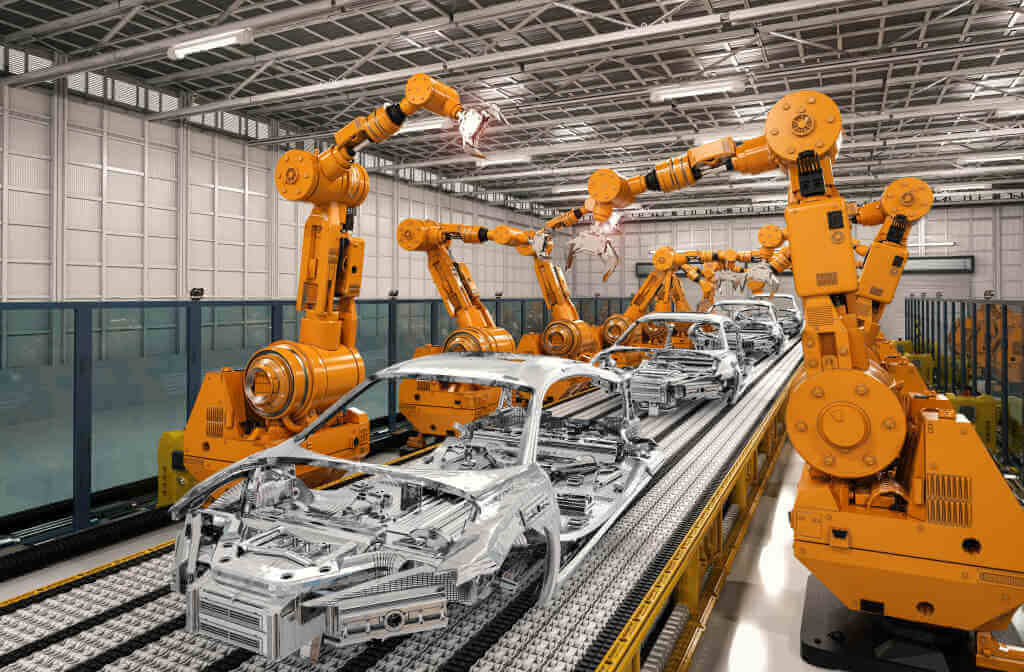
\includegraphics[width=10cm]{figures/IndustrialRobot.jpg}
  \caption[Robot công nghiệp]{Robot công nghiệp [Nguồn: Internet]}
  \label{fig:RBCongNghiep}
\end{figure}

\section{codeword}

Ví dụ về font \codeword{code}

\section{code section}

Ví dụ về đoạn code

\begin{lstlisting}[numbers=none, language=bash]
	sudo apt-get install -y chrony ntpdate
	sudo ntpdate -q ntp.ubuntu.com
\end{lstlisting}
% \input{chapters/chapter34}
% ----- Draft --------------------
% \input{chapters/draft_reviewPapers}

% ----Tài liệu tham khảo-----------------------------
% \bibliographystyle{plain}
\bibliographystyle{ieeetr}
\bibliography{ref.bib}
% ==============================
\end{document}

%%% Local Variables:
%%% mode: latex
%%% TeX-master: t
%%% End:
